\documentclass[a4paper,titlepage]{article}

\usepackage[english]{babel}
\usepackage[utf8]{inputenc}
\usepackage{graphicx} 
\usepackage[T1]{fontenc}
\usepackage{datetime}
\usepackage{hyperref}
\usepackage{hyperxmp}
\usepackage{url}

\author{
	Clodéric Mars - Golaem \\ 
	\small \href{mailto:cloderic.mars@gmail.com}{cloderic.mars@gmail.com}\\
	\small \href{http://www.crowdscontrol.net}{www.crowdscontrol.net} -- \href{http://www.golaem.com}{www.golaem.com}}
\title{Group navigation state-of-the-art report}
\date{}

\newcommand{\sectionsubtitle}[1]{{\subsection*{\scshape #1}}} 

\hypersetup{
pdftitle={Group navigation state-of-the-art report},
pdfauthor={Clodéric Mars <cloderic.mars@gmail.com>},
pdfcopyright={This work is licensed under a Creative Commons Attribution-NonCommercial-ShareAlike 3.0 Unported License},
pdflicenseurl={http://creativecommons.org/licenses/by-nc-sa/3.0/},
pdfkeywords={autonomous agents navigation, crowd simulation},
pdflang={en}
}

\graphicspath{{./figures/}}

\begin{document}

\maketitle

\tableofcontents

\section*{History}
\begin{tabular}{|l|p{8cm}|}
\hline
\dmyyyydate{\formatdate{21}{6}{2011}} & Initial version.\\ \hline
\dmyyyydate{\formatdate{17}{9}{2011}} & First final \LaTeX version. \\ \hline
\end{tabular}

\section*{License}
This work is licensed under the Creative Commons Attribution-NonCommercial-ShareAlike 3.0 Unported License. To view a copy of this license, visit \url{http://creativecommons.org/licenses/by-nc-sa/3.0/} or send a letter to Creative Commons, 444 Castro Street, Suite 900, Mountain View, California, 94041, USA.

\pagebreak
\section{Introduction}
\label{sec:introduction}

Autonomous human-like characters being able to navigate in a 3D environment finding their paths and avoiding collisions while exhibiting a convincing behavior is now fairly common. The popularity and the quality of recent work \cite{vandenBerg:2008tu,Pettre:2009tg,Ondrej:2010we,Mononen:2010wp} shows that the simulation of hundreds of navigating entities is now within the reach of almost everyone. But most of these work focus on simulating lonely entities taking their neighbors into account only to avoid collisions. Like real ones, our virtual humans should be able to walk down the road with their group of friends. Like real ones, our virtual soldiers must be able to march on enemy positions while staying in formation. And like real ones, our virtual tourists have to be able to enjoy their tour of the Mont Saint-Michel following their guide’s umbrella.

Before we start designing and implementing group navigation behaviors in Golaem Path \cite{GolaemPath:tw}, let’s first see what others have done. This document is a state-of-the-art study of existing work concerning group and formations navigation with a focus on algorithms and implementations. The first part defines the different categories of navigating groups we’re interested in. The second section focuses on how the group members can stay grouped or in formation during navigation. The third and last section talks about the group’s navigation from path planning to steering and collision avoidance.

\section{Taxonomy}
\label{sec:taxonomy}
\sectionsubtitle{Aka "flocks, herds and school" and...}

Before we talk velocity, steering behaviors and gradient descent, let’s first present the kind of groups we’re trying to make navigate, their characteristics and their constraints. In this section we’ll divide navigating groups in three categories, flocks, formations and small groups resulting of social influences.

\subsection{Flocks}
\label{sec:taxonomy:flocks}

\begin{figure}[h]
\centering
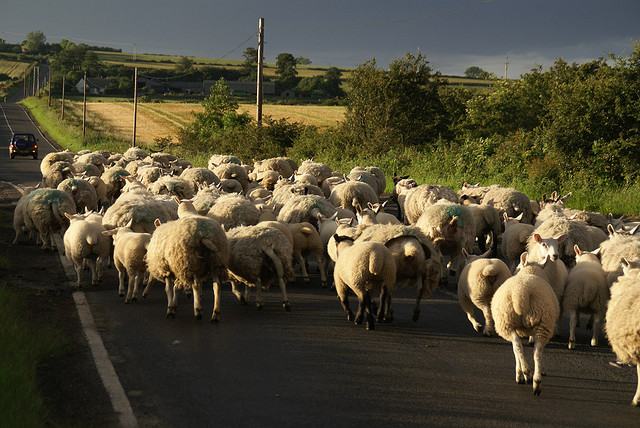
\includegraphics[width=0.9\textwidth]{SheepsHerd.jpg}
\caption{Sheep flock (from~\url{http://flic.kr/p/Yuy89}).}
\label{fig:sheep_flock}
\end{figure}

A flock is primarily a group of bird traveling together but it can be applied to other animal species (cf.\ figure~\ref{fig:sheep_flock}) as well as humans (e.g.\ a flock of school children is crossing the street to the swimming pool). Entities in a flock travel at roughly the same speed and form a cohesive group without strict arrangement. In what must be the two most cited articles in the field \cite{Reynolds:1987vm,Reynolds:1999vr}, Reynolds studied empirically how flocks members move relatively to each others. With simple behaviors he was able to recreate a flock of autonomous entities, we’ll dig into more details in section~\ref{sec:stay_grouped:emergence}.

\subsection{Formations}
\label{sec:taxonomy:formations}

\begin{figure}[h]
\centering
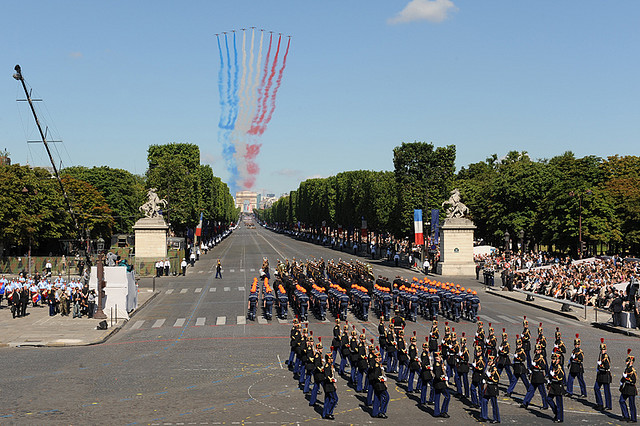
\includegraphics[width=0.9\textwidth]{BastilleDay.jpg}
\caption{Foot soldiers in formations for the Bastille day military parade (from~\url{http://flic.kr/p/57KrxH}).}
\label{fig:bastille_day}
\end{figure}

While flocks do not follow more rules than the cohesion of the group, formations are a kind of group arrangement where members need to enforce strict rules. Both in a combat or a parade (cf.\ figure~\ref{fig:bastille_day}), the spatial arrangement, i.e. the relative positions of members, is designed for a precise purpose, tactic or aesthetic; it is the first rule that needs to be followed. Secondly, in a combat context, formation gets much of its usefulness from overlapping fields of fire and sight, that’s why the orientation is another rule to be followed \cite{Dawson:2002vd}. The last rule is to assign entities having the right role to the right slot: archers at the back, footsoldiers facing the enemy. As navigation and military simulation are important for real time strategy games, interesting and working solutions has been developed early: Dave Pottinger, who worked on the Age of Empire series, presented his in a Gamasutra article \cite{Pottinger:1999vk}.

\subsection{Small social groups}
\label{sec:taxonomy:small_social_groups}

\begin{figure}[h]
\centering
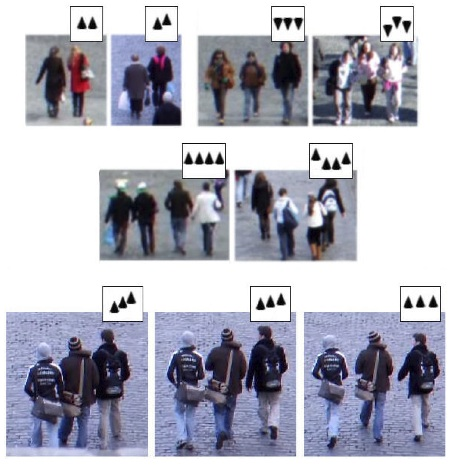
\includegraphics[width=0.7\textwidth]{SocialGroups.jpg}
\caption{Examples of groups of two, three and four (from~\cite{Peters:2009kx}).}
\label{fig:social_groups}
\end{figure}

\begin{figure}[h]
\centering
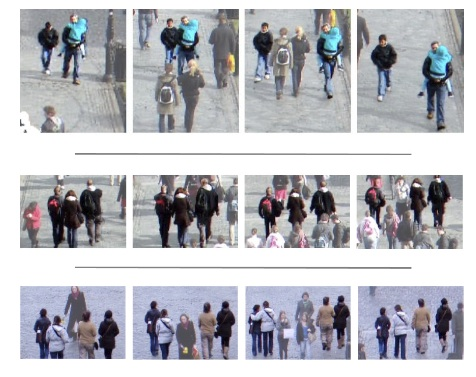
\includegraphics[width=0.7\textwidth]{SocialGroupsSplitting.jpg}
\caption{Examples of groups of two, three and four splitting to avoid collison (from \cite{Peters:2009kx}).}
\label{fig:social_groups_splitting}
\end{figure}

Beyond amorphous flocks and rigid military formations, groups that are more common in our everyday life are small and their spatial configuration is the result of social factors and crowd density. Two recent survey focuses on those small social groups \cite{Peters:2009kx,Moussaid:2010ib}, they lead to the same conclusions.
The two studies were conducted from videos taken at public spaces (in France and Ireland). Their observations show that: there are more groups than single pedestrians, groups of more than four are very rare and most of the groups are, indeed, pairs.

More interesting, it appears the formation adopted by the observed groups is influenced both by the lateral clearance to nearby obstacles and by the social interaction between members of the group (cf.\ figure~\ref{fig:social_groups}). When motion is not constrained (i.e.\ when obstacles are far and the crowd density is low) a group tends to adopt an abreast formation that facilitates dialog between its members. When facing navigation constraints, to reduce its frontal width, the group compact the formation. And when the lateral space between each member become too thin, i.e.\ when members are shoulder-to-shoulder, the formation is staggered. The bending of the group is, most of the time, forward (V-like formation) to maintain good communication when a backward bending (inversed-V-like or wedge formation) would be more flexible moving against an opposite flow.

Finally, while groups tend to avoid collisions, with other pedestrians or with obstacles, as a whole they are able to split if needed merging back afterwards (cf.\ figure~\ref{fig:social_groups_splitting}).

\section{Stay Grouped!}
\label{sec:stay_grouped}
\sectionsubtitle{How members enforce group constraints}

In order to get a valid simulation of group navigation we first have to design the behavior of the group members. In this section we’ll study two families of methods to obtain groups: using local rules or following a designed formation. Finally we’ll focus on how a member’s individual navigation behavior is affected when part of a group.

\subsection{Emergence}
\label{sec:stay_grouped:emergence}

In most modern navigation engine, the simulated entities are autonomous, their behavior rely on their local "perception” to take action not on an external choreographer. With this approach in mind, several works relies on decentralized behavior to enforce group constraints.

\subsubsection{Flocking}

At the core of Reynolds’ work \cite{Reynolds:1987vm,Reynolds:1999vr}, three steering behaviors (cf.\ figure~\ref{fig:flocking_steering_behaviors}) allows entities to flock. For any given entity in the group, separation makes him move apart too close neighbors, alignment makes him go in the same direction as other members and cohesion makes him move towards the group’s COM (center of mass). These simple behaviors allow the emergence of a flock. Others took inspiration from this work and adapt it to their architecture using voting steering behaviors \cite{Hostetler:2002wg} or relying on specific environment abstraction such as grids \cite{Loscos:2003wh} or roadmaps \cite{Bayazit:2003up,Kamphuis:2004ct}.

\begin{figure}[h]
\centering
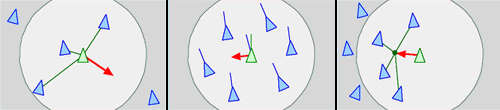
\includegraphics[width=\textwidth]{FlockingSteeringBehaviors.jpg}
\caption{Flocking steering behaviors, from left to right: Separation, Alignment and Cohesion (from~\cite{Reynolds:1999vr}).}
\label{fig:flocking_steering_behaviors}
\end{figure}

\subsubsection{Social relations}

In his recent paper, Moussaïd \cite{Moussaid:2010ib}, extends the social force model \cite{Helbing:2000vh} to obtain flocking as well as more structured small formation introducing a communication force. The gaze of group members is attracted by the center of interest of the group; here its center of mass (COM) is used. The communication force tries to limit the gaze deviation by decelerating the entity thus enabling the observed V-like formation (cf.\ section~\ref{sec:taxonomy:small_social_groups}).

In order to take into account social relations between members of the group, Qiu uses a member-to-member influence matrix \cite{Qiu:2010ks}. This matrix is taken into account when computing the attraction between members of the group. This approach allows the definition of one or more attractive (or repulsive) members of the group such as more talkative persons or tourist guides.

\subsubsection{More rigid formations}

Local rules can also exhibit a more strict formation. Taking inspiration from molecular crystals, Balch and Hybinette designed the attachment sites method \cite{Balch:2000bn}. Each entity, given its desired formation, computes several attachment sites on its neighbors (cf.\ figure~\ref{fig:attachment_sites}) and steers to reach the nearest available. The resulting formation arrangement is a direct result of the attachment sites position and it can scale to any number of group members. But as the attachment rules are local, no control on the formation overall shape is possible. 

\begin{figure}[h]
\centering
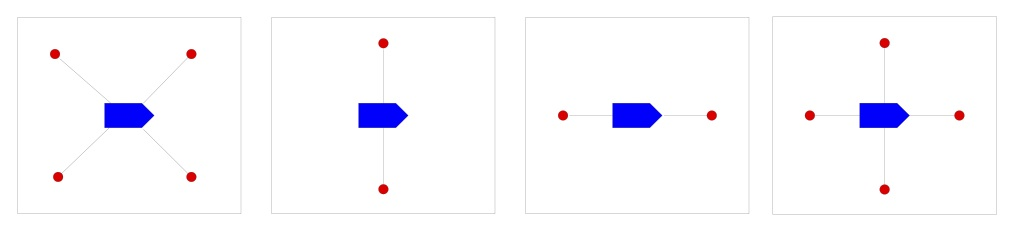
\includegraphics[width=\textwidth]{AttachmentSites.jpg}
\caption{Blue entities and different red attachment sites (from~\cite{Balch:2000bn}).}
\label{fig:attachment_sites}
\end{figure} 

\subsection{Choreography}
\label{sec:stay_grouped:choreography}

While groups whose members are implementing local rules can exhibit convincing behavior, they can’t take into account the group as a whole and thus are not fully controllable. If an exact group arrangement is needed, some of the behavior must be deported to an upper level of control \cite{MusTha2001}. In this part we’ll study the three features needed to make a group stay in a given formation: the formation design, the slot assignment and the formation hold.

\subsubsection{Design}

A formation is basically a list of slots to which members of the group will be assigned. As we focus on pedestrian navigation, a slot is basically a 2D position relative to the group “center”. In a military context two properties of the slot must be added, as we saw in section \ref{sec:taxonomy:formations}: the orientation and the role (i.e.\ which kind of entity should be assigned to this slot).

Such a formation definition can be designed manually following military principles or artistic concerns \cite{Dawson:2002vd}.  Another approach has been taken by Karamouzas and Overmars \cite{Karamouzas:2010fi}, they extracted from the data collected by Moussaïd et al. \cite{Moussaid:2010ib} a set of typical formations for small social groups of 2 to 4 members. The figure~\ref{fig:social_group_formations} shows the three kinds of formations they get for groups of 3; similar formations are obtained for groups of 2 or 4. 

\begin{figure}[h]
\centering
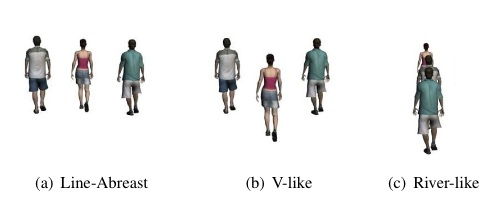
\includegraphics[width=0.8\textwidth]{SocialGroupFormations.jpg}
\caption{Three members social group formations (from~\cite{Karamouzas:2010fi}).}
\label{fig:social_group_formations}
\end{figure} 

\subsubsection{Assign}
We now assume the formation design is chosen and defines as many slots as group members; if not, simple techniques can be used to select the used slots or create needed slots \cite{Silveira:2008bc}. The next needed step before our entities can navigate as a group, is to assign each of them to a slot. This part might seem trivial but should be implemented right to avoid destroying the simulation credibility with traffic jams between members of the same groups.

Implementation-oriented papers \cite{Dawson:2002vd,Millington:2006wz} describe different solutions and their quality. As everyone should expect, random or index-based (i\textsuperscript{th} members with i\textsuperscript{th} slot) assignment are most of the time really bad: the entities might have to cross each others and to circle around the group to get to their slot. To avoid this bad result, one solution could be to, sequentially assign to each entity, its closest free spot, this solution is easy to implement and might work but last entities might end up to far slots as the closest one are already taken. The best solutions would be to globally minimize the distance the entities are covering to get to their slots but its implementation would lead to an $O(n!)$ complexity as every permutation would have to be tested. 

One solution to get a good result and keep a good complexity is a two steps process. First compute for each members of the group what is their cost to be assigned to which slot, allowing certain slot to be specialized for certain entity roles. Then, from the most expensive to assign to the cheapest assign entities to their preferred available slot. This solution might fail to get the optimal assignment but should have decent result while keeping a low complexity $O(n^2)$
\cite{Millington:2006wz}.

Another solution works only when no specialized slots are defined. Given a formation design, first sort the slots spatially; for a horizontal line formation, the slot might be sorted from left to right along a horizontal vector. Then sort the group members in the same way; finally assign the i\textsuperscript{th} entity to the i\textsuperscript{th} slot \cite{Dawson:2002vd}.

\subsubsection{Maintain}

The formation being built, entities are able to reach their slots and to arrange into the designed formation. Let’s see how they are able to maintain it while the group is moving.

In earlier work \cite{Pottinger:1999vk}, a simplistic approach is taken: once part of a formation, entities are no longer responsible for their steering, their position is set at each time step according to the formation. This solution is fine if the group steering (cf.\ section~\ref{sec:who_s_in_charge}) is robust enough to handle the desired level of collision avoidance.
Using the latter solution, the members do not have an own steering behavior: it is difficult to get anything but a strictly followed formation. To allow formations of individuals, several works uses a more loose approach, members are given a local goal to reach in order to stay in formation and are in charge of fulfilling this goal. A simple approach is to provide each member with a simple “reach target” steering behavior where the target is its slot’s future position \cite{Karamouzas:2010fi,Schuerman:2010um}. This approach works better if the slots are within navigable space as shown in Schuerman et al. videos. To avoid this problem, Silveira, Prestes and Nedel define a group potential map using slots as attractors and obstacles as repulsors thus providing to members a velocity that maintain the formation while keeping a smooth path when obstacle are present. It allows entity to break formation to pass through tight corridors and around small obstacles \cite{Silveira:2008bc}.

\subsection{Group members steering}
\label{sec:stay_grouped:group_members_steering}

Whether the group is a flock or a formation, the individual steering behaviors, the collision avoidance in particular, of its members has to be considered. We’ve seen that in some case the individual steering behaviors are disabled \cite{Pottinger:1999vk}. In most work though, the group navigation is designed to work in conjunction with its members’, the main problematic is to blend the individual behavior with the group orders.

In some architecture, each entity has several independent behaviors producing different steering orders that are blended together using weight and priorities. In this kind of approach the group orders are executed by another behavior and are part of the final blend \cite{Moussaid:2010ib,Qiu:2010ww,Hostetler:2002wg}. 

In most modern architecture, a pipeline of behaviors produce a steering order each element taking the previous into account while enforcing new constraints or orders, the last one being collision avoidance \cite{GolaemPath:tw,Mononen:2010wp}. The group orders are implemented as a part of this pipeline, they are fed to the following elements among which the collision avoidance \cite{Karamouzas:2010fi,Silveira:2008bc}. 

Schuerman et al. state that while the same collision avoidance behavior can be used by the entities when they are part of a group, it must be adapted. As a matter of fact, collision avoidance algorithms such as RVO \cite{vandenBerg:2008tu} try to enforce a safe distance to obstacles and other entities that might forbid tight formations. A “boldness” factor is introduced controlling how likely an entity is to yield to other entities during steering. When a strict formation is desired the “boldness” factor of its members is set high making them only try to avoid imminent collisions \cite{Schuerman:2010um}.

\section{Who's in charge?}
\label{sec:who_s_in_charge}
\sectionsubtitle{Group level decision making}

In the previous part, we studied how group members are able to maintain cohesion or stay in formation. In this part, we’ll study how the group, a whole, is able to make navigation decisions: path planning, path following, steering (including collision avoidance) and formation changes. 

\subsection{Anchor}
\label{sec:who_s_in_charge:anchor}

While some behavior might be decentralized (cf.\ section~\ref{sec:stay_grouped:emergence}), in order to leverage groups in a context where we need to make them go from A to B, top-down decision making is needed \cite{MusTha2001}. A group level process will be able to make the group move while each of its member follows. 
We call anchor a virtual object that group members use as a reference for their formation or flocking behaviors and to which they delegate some navigation processes. It aggregates various data relative to the group, such as its position, orientation and velocity and it’s where the group level decision-making is done.

\subsubsection{Leader}

Trying to enforce a strict equivalence between simulated entities and actual characters, lots of works rely on a leader-followers approach. In such approach, one member of a group is the leader where the others are the followers. The leader takes responsibility for the whole group regarding the navigation; it becomes the anchor of the group \cite{Loscos:2003wh,Qiu:2010ks}.

The implementation of such an approach using a navigation engine for independent entities is straightforward: the leader is similar to an independent entity; while the followers uses a subset of the default processes and maintain a reference to their leader.

But the leader can’t reuse the exact same processes of an independent entity. Its navigation must take into account the bulk of the whole group as well as the different locomotion constraints of its followers. It is also better to differentiate the the leader’s own attributes (position, orientation and velocity) from the anchor’s \cite{Millington:2006wz}. Taking all these constraints into account makes the decision-making process of the leader very different from the other members.

\subsubsection{Group entity}

Noting that the leader-based approach as several flaws, a growing proportion of architectures chose to move the group anchor from the leader to a virtual group entity \cite{Schuerman:2010um,Silveira:2008bc,Karamouzas:2010fi}. This virtual entity is similar to any other simulated entities but doesn’t have visual or physic (i.e. regarding collision detection) representation. In such architecture, the group members are identical to one another. 
In Schuerman et al. \cite{Schuerman:2010um} work, other entities detect groups entities during their collision avoidance process, trying to avoid collisions with groups as the whole. Entities are thus able to simulate the fact that pedestrians tend to avoid to pass through a group.

The group entity creates a one level deep hierarchy of entities. This approach can be taken a step further to create groups of groups and so on \cite{Schuerman:2010um,Millington:2006wz} allowing a more structured crowd.

\subsection{Path planning/following}
\label{sec:who_s_in_charge:path_planning_following}

One of the reasons for group navigation is to factorize a costly aspect of navigation: path planning. As a matter of fact the members of a group are expected to follow the same high-level path through the environment, a single query should be sufficient for the whole group.

The most important aspect of group level path planning is to choose how to take the bulk of the group into account.  Contrary to a single entity where its bulk can’t be changed and thus is a hard constraint, a group can reconfigure in order to pass through narrower corridors. The query has to be tuned in order to prefer paths on which the group, in its current spatial configuration, can navigate but be able to select narrow passages if necessary. This implies that the cost of falling back to a narrower spatial configuration can be compared to the cost of taking a longer path \cite{Kamphuis:2004ct,Pottinger:1999vk,Bayazit:2003up}.

Once the path is computed, the path following process is able to provide local steering orders resulting in the entity following the path. Adapted to groups, this process makes the anchor follow the path. In some work \cite{Bayazit:2003up,Pottinger:1999vk}, the group level path following is also responsible for environment aware formation adaptation, allowing the formation to change when the clearance to obstacles changes. The figure~\ref{fig:narrow_passage} shows how a formation change allows a group to pass through a narrow passage more smoothly.

\begin{figure}[h]
\centering
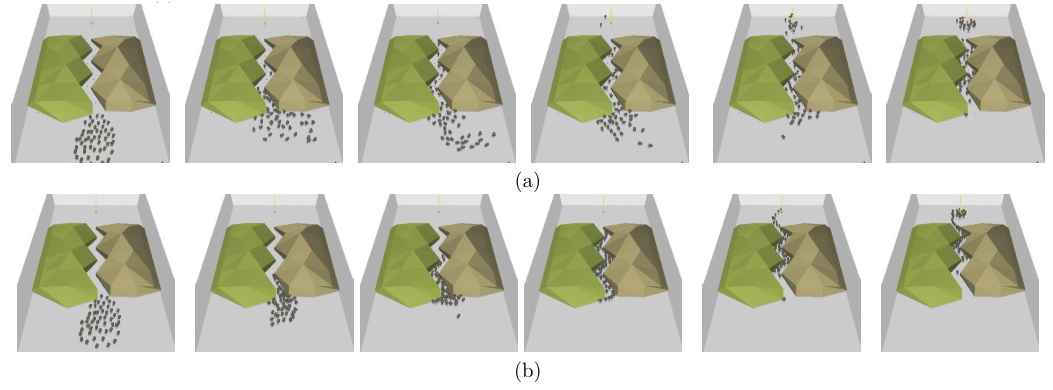
\includegraphics[width=\textwidth]{NarrowPassage.jpg}
\caption{Passing through a narrow passage using flocking (a) or river-like formation (b) (from~\cite{Bayazit:2003up}).}
\label{fig:narrow_passage}
\end{figure} 

\subsection{Collision avoidance}
\label{sec:who_s_in_charge:collision_avoidance}

Groups tend to stay coherent when navigating between obstacles and among other pedestrians, that’s why several work features group level collision avoidance. Numbers of existing algorithm for entities can be applied directly or adapted for group level collision avoidance. As we noted for path planning and following, the main difference between groups and single entities is that their bulk is not a hard constraint. The spatial configuration of a group can be adapted to occupy less frontal space, less longitudinal space or both. 

Schuerman et al.\ consider the bulk of the group as a disc allowing them to use RVO \cite{Schuerman:2010um,vandenBerg:2008tu}. The resulting collision avoidance is very conservative as the disc is, most of time greatly overestimating the real footprint of the group. Karamouzas and Overmars adapted their own collision avoidance algorithm, based on velocity space sampling and sweep collision test, to work on the oriented bounding box of the group \cite{ko_vriphys10,Karamouzas:2010fi}. They further extend the algorithm by allowing formation adaptation. In practice, they generate samples based on velocity changes and formation changes interpolating the current formation with a library of valid formation (cf.\ figure~\ref{fig:formations_linear_interpolation}). Each sample is weighted depending on its distance from the desired velocity and the desired formation and its time to collision. The number of candidate formations is limited to 15 as there’s 5 possible formations and 3 interpolations computed per formation. These limits lower the number of considered samples, preserving the performances of the algorithm. 

\begin{figure}[h]
\centering
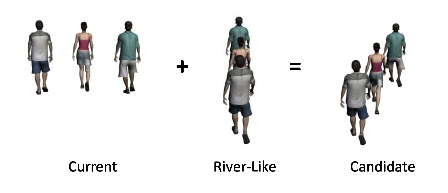
\includegraphics[width=0.8\textwidth]{FormationsLinearInterpolation.jpg}
\caption{Linear interpolation between formations (from~\cite{Karamouzas:2010fi}).}
\label{fig:formations_linear_interpolation}
\end{figure} 

Peters et al. rule based navigation method is able to handle both formation adaptation and group splitting which is not supported by the previously described methods \cite{Peters:2009kx}. Unfortunately the article doesn’t provide many details on the algorithm.

Those group level navigation methods allows the group to take responsibility for a part of collision avoidance and more easily preserve the group cohesions. The members’ own navigation behaviors are still necessary both to preserve individual behaviors and to avoid remaining collisions. 

\section{Conclusion}
\label{sec:conclusion}

This review was limited to the navigation aspect of the group, it is supposed to answer to the question: \emph{“How to make a group navigate in my simulation/game?”}. A group is, most of the time, the result of social interactions and relations between individuals that have other consequences beyond navigation strategy: body language, facial expressions, and speech… For a simulated group to be believable those other aspects must be addressed.

This state-of-the art study was instrumental in the design of Golaem Path upcoming group navigation features \cite{GolaemPath:tw}. I hope others developers or even researchers in the field will find it useful. I’ll try to update its content as other works come to my knowledge or are published.

\pagebreak
\bibliographystyle{alphaurl}
\bibliography{Group_navigation_state-of-the-art_report}

\end{document}
